\documentclass[paper=a4, fontsize=11pt]{scrartcl} % KOMA-article class

%-------------------------------------------------
%   THEMES, PACKAGES, CUSTOM COMMANDS
%-------------------------------------------------
\usepackage{blindtext}
\usepackage[english]{babel}                             % English language/hyphenation
\usepackage[protrusion=true,expansion=true]{microtype}  % Better typography
\usepackage{amsmath,amsfonts,amsthm,mathtools}                    % Math packages
\usepackage[pdftex]{graphicx}                           % Enable pdflatex
\usepackage[export]{adjustbox}
\usepackage[svgnames]{xcolor}                           % Enabling colors by their 'svgnames'
\usepackage[hang, small,labelfont=bf,up,textfont=it,up]{caption} % Custom captions under/above floats
\usepackage{subcaption}
\usepackage{epstopdf}       % Converts .eps to .pdf
%\usepackage{subfig}         % Subfigures
\usepackage{booktabs}       % Nicer tables
\usepackage{fix-cm}         % Custom fontsizes
\usepackage{listings}
\usepackage{soul}
\usepackage{hyperref}
\usepackage[backend=bibtex]{biblatex}
\usepackage{filecontents}

\usepackage[foot=30pt,margin=1in]{geometry}

% Custom sectioning (sectsty package)
\usepackage{sectsty}
\allsectionsfont{
    \usefont{OT1}{phv}{b}{n}    % bch-b-n: CharterBT-Bold font
}
\sectionfont{
    \usefont{OT1}{phv}{b}{n}
}

% Custom colors
\definecolor{brsugrey}{rgb}{0.9, 0.9, 0.9}
\definecolor{brsublue}{rgb}{0, 0.594, 0.949}

%
\newcommand{\upperRomannumeral}[1]{\uppercase\expandafter{\romannumeral#1}}

% Creating an initial of the very first character of the content
\usepackage{lettrine}
\newcommand{\initial}[1]{%
    \lettrine[lines=3,lhang=0.3,nindent=0em]{
        \color{brsublue}
        {\textsf{#1}}}{}}

%-------------------------------------------------
%   COMMON INFO
%-------------------------------------------------
\newcommand{\hmwkTitle}{Homework 3}
\newcommand{\hmwkDueDate}{Lecture date: 17 October 2016}
\newcommand{\hmwkClass}{Neural Networks}
\newcommand{\hmwkClassShort}{NN WS2016}
\newcommand{\hmwkAuthorFullName}{Minh H. Nguyen and Padmaja Kulkarni}
\newcommand{\hmwkAuthorLastName}{Nguyen \& Kulkarni}
\newcommand{\hmwkAuthorEmail}{minh.nguyen@smail.inf.h-brs.de}
\newcommand{\hmwkAuthorInstitute}{BRS University of Applied Sciences}

%-------------------------------------------------
%   HEADERS & FOOTERS
%-------------------------------------------------
\usepackage{fancyhdr}
\pagestyle{fancy}
\usepackage{lastpage}
% Header (empty)
\lhead{}
\chead{}
\rhead{}
% Footer (you may change this to your own needs)
\lfoot{\footnotesize
    \texttt{\hmwkClassShort} ~
    \textbullet ~ \hmwkAuthorLastName ~
    \textbullet ~ \hmwkTitle}
\cfoot{}
\rfoot{\footnotesize page \thepage\ of \pageref{LastPage}}  % "Page 1 of 2"
\renewcommand{\headrulewidth}{0.0pt}
\renewcommand{\footrulewidth}{0.4pt}

%-------------------------------------------------
%   TITLE & AUTHOR
%-------------------------------------------------
\usepackage{titling}

\newcommand{\HorRule}{\color{brsublue}% Creating a horizontal rule
    \rule{\linewidth}{1pt}%
    \color{black}
}

% Title
\pretitle{
    \begin{flushleft}
        \HorRule
        \fontsize{25}{25} \usefont{OT1}{phv}{b}{n} \color{gray} \selectfont
}
\title{\hmwkClass \\
       \hmwkTitle}
\posttitle{
    \par
    \end{flushleft}
}

% Author
\preauthor{
    \begin{flushleft}
        \large \lineskip 0.25em
        \usefont{OT1}{phv}{b}{sl} \color{brsublue}}

\author{\hmwkAuthorFullName}

\postauthor{
        \footnotesize
        \usefont{OT1}{phv}{m}{sl} \color{Black}
        \\\hmwkAuthorInstitute
        \\\hmwkAuthorEmail
        \par
    \end{flushleft}
    \HorRule}

% Date
\date{\hmwkDueDate}

\begin{filecontents*}{homework.bib}
    @article{mead1990,
        title={Neuromorphic electronic systems},
        author={Mead, Carver},
        journal={Proceedings of the IEEE},
        volume={78},
        number={10},
        pages={1629--1636},
        year={1990},
        publisher={IEEE}
    }
\end{filecontents*}

\bibliography{homework}

%-------------------------------------------------
%   BEGIN
%-------------------------------------------------
\begin{document}
    \maketitle
    \thispagestyle{fancy} % Enabling the custom headers/footers for the first page

    \section*{Problems}

    \subsection*{Problem 2-1}
    {
    \def\arraystretch{1.5}
    \begin{tabular}{| p{3.5cm} | p{5.5cm} | p{5.5cm} |}
        \hline
                    & Delta rule & Hebb's hypothesis (activity product rule) \\
        \hline
        Equation    & $ \Delta w_{kj}(n) = \eta e_k(n) x_j(n) $ & $ \Delta w_{kj}(n) = \eta y_k(n) x_j(n) $ \\
        Weight adjustments depend on
                    & error signal (difference between desired target and actual output), input signal
                    & output signal and input signal \\
        Paradigm    & supervised (depends on how to define ``desired'' outputs)
                    & unsupervised (learning purely depends on data) \\
        Stability   & similar to closed loop feedback system, depends on learning rate
                    & $\Delta w_{kj}(n)$ grows exponentially if constant input is applied \\
        \hline
    \end{tabular}
    }

    \subsection*{Problem 2-10}

    \begin{center}
    \setlength{\fboxsep}{0.5pt} %
    \setlength{\fboxrule}{0.5pt} %,fbox
    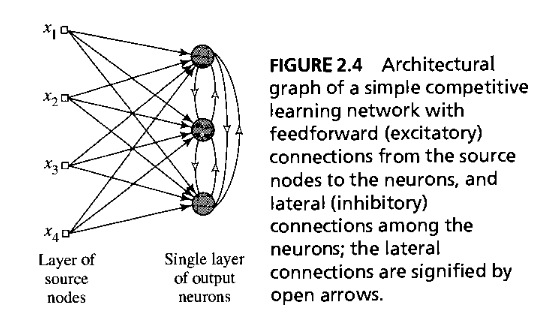
\includegraphics[width=10.0cm]{../images/Haykin-NN-figure2-4.png} %
    \end{center}

    Output $y_j$ of neuron $j$:
    \[ v_j = \sum_i w_{ji} x_i + \sum_k c_{kj} y_k = \sum_i w_{ji} x_i + \sum_k c_{kj} \sum_i w_{ki} x_i \]
    \[ y_j = \phi(v_j) = \phi \left( \sum_i w_{ji} x_i + \sum_k c_{kj} \sum_i w_{ki} x_i \right) \]
    Neuron $j$ is winning if $v_j$ is larger than local fields of all other neurons.

    \subsection*{Problem 2-21}

    \begin{center}
        \setlength{\fboxsep}{0.5pt} %
        \setlength{\fboxrule}{0.5pt} %,fbox
        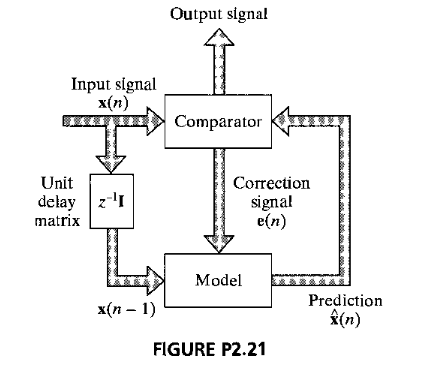
\includegraphics[width=10.0cm]{../images/Haykin-NN-figurep2-21.png} %
    \end{center}

    Comments on the system:
    \begin{itemize}
        \item From \cite{mead1990}, the above model resembles a neural processing system, in which only wrong predictions are used for adjusting the model and sending to the central nervous system and correct predictions are ignored.
        \item Number of time steps $m$ has to be of a time window long enough for the input data to be considered pseudo-stationary (from section 2.12).
        \item The system tries to predict the input itself, instead of a separated signal.
        \item There's no weight matrix for the input vector.
        \item The system resembles both error correction learning because of the adaptation to prediction error, and Boltzmann machines because of the recurrent element.
    \end{itemize}

    \newpage
    \subsection*{Question 5}
    Result of running the attached Python script inspired by a tutorial by Edwin Chen (\href{http://blog.echen.me/2011/07/18/introduction-to-restricted-boltzmann-machines/}{link}):

    \begin{lstlisting}
initial weights are:
[[ 0.98420826  0.67334206  0.72858161]
[ 0.37161027  0.16045081  0.91969487]] 

Updated weights are:

[[ 0.95634999  0.64958522  0.69383697]
[ 0.34602563  0.13857249  0.89953725]]
    \end{lstlisting}


    \printbibliography

\end{document}
